% Body of the App Store screenshot decks (store-en/de/fr.tex): a short lecture
% with figures, a formula and a table, notes on the right (keyword SP-Right).
% Before \input, define \storelang to en, de or fr. All text is in this file,
% so the three decks only differ in language.
\documentclass[aspectratio=169]{beamer}
\input{common/preamble}
\usepackage[T1]{fontenc}
\usepackage{lmodern}
\usepackage{pgfpages}
\usepackage{tikz}
\usepackage{booktabs}
\usetikzlibrary{calc}
\setbeameroption{show notes on second screen=right}

\definecolor{spblue}{RGB}{0,102,204}
\definecolor{sporange}{RGB}{230,120,0}
\setbeamercolor{frametitle}{fg=spblue}
\setbeamercolor{title}{fg=spblue}
\setbeamercolor{structure}{fg=spblue}
\setbeamertemplate{navigation symbols}{}
\setbeamerfont{note page}{size=\Large}
% Notes page: only the notes, no title, date or slide thumbnail.
\setbeamertemplate{note page}{\vspace*{1.5em}\usebeamerfont{note page}\insertnote}

% \L{en}{de}{fr} picks the text of the deck's language.
\def\L#1#2#3{\csname L@\storelang\endcsname{#1}{#2}{#3}}
\makeatletter
\def\L@en#1#2#3{#1}
\def\L@de#1#2#3{#2}
\def\L@fr#1#2#3{#3}
\makeatother

\title{\L{Kepler's Laws}{Die Keplerschen Gesetze}{Les lois de Kepler}}
\subtitle{\L{How planets move around the Sun}{Wie sich Planeten um die Sonne bewegen}{Comment les planètes tournent autour du Soleil}}
\hypersetup{pdftitle={\L{Kepler's Laws}{Die Keplerschen Gesetze}{Les lois de Kepler}}, pdfkeywords={SP-Right}}

\begin{document}

\begin{frame}
  \titlepage
  \vspace{-2.5em}
  \centering
  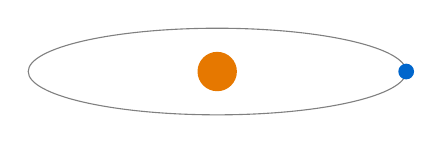
\begin{tikzpicture}
    \fill[sporange] (0,0) circle (0.25);
    \draw[gray] (0,0) ellipse (2.4 and 0.55);
    \fill[spblue] (2.4,0) circle (0.1);
  \end{tikzpicture}
\end{frame}
\note{\L{%
  \begin{itemize}
    \item Welcome, introduce the topic
    \item Kepler published the first two laws in 1609
    \item Ask: who has seen an orbit drawn as a circle?
  \end{itemize}}{%
  \begin{itemize}
    \item Begrüßung, Thema vorstellen
    \item Kepler veröffentlichte die ersten beiden Gesetze 1609
    \item Frage: Wer hat eine Umlaufbahn schon als Kreis gesehen?
  \end{itemize}}{%
  \begin{itemize}
    \item Accueil, présenter le sujet
    \item Kepler publie les deux premières lois en 1609
    \item Question : qui a déjà vu une orbite dessinée en cercle ?
  \end{itemize}}}

\begin{frame}{\L{First law: orbits are ellipses}{Erstes Gesetz: Bahnen sind Ellipsen}{Première loi : les orbites sont des ellipses}}
  \centering
  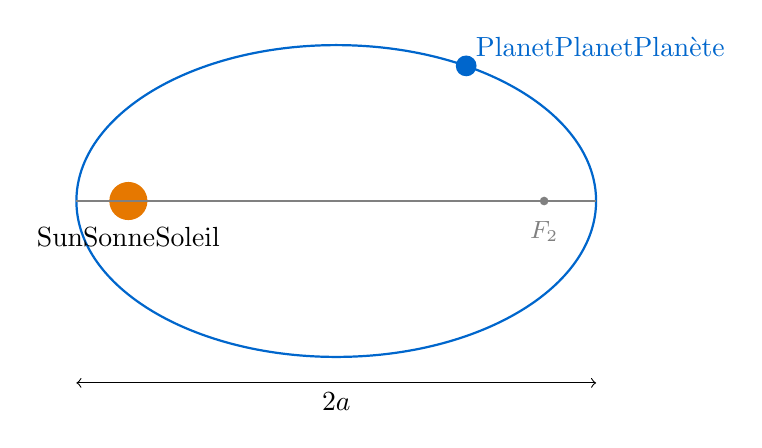
\begin{tikzpicture}[scale=1.1]
    \draw[thick, spblue] (0,0) ellipse (3 and 1.8);
    \fill[sporange] (-2.4,0) circle (0.22) node[below=6pt, black] {\L{Sun}{Sonne}{Soleil}};
    \fill[gray] (2.4,0) circle (0.05) node[below=4pt] {\small $F_2$};
    \fill[spblue] (1.5,1.56) circle (0.12) node[above right] {\L{Planet}{Planet}{Planète}};
    \draw[gray] (-3,0) -- (3,0);
    \draw[<->] (-3,-2.1) -- node[below] {$2a$} (3,-2.1);
  \end{tikzpicture}
\end{frame}
\note{\L{%
  \begin{itemize}
    \item The Sun is in one focus, not in the center
    \item Earth's orbit is almost a circle: eccentricity 0.017
    \item $a$ is the semi-major axis
  \end{itemize}}{%
  \begin{itemize}
    \item Die Sonne steht in einem Brennpunkt, nicht in der Mitte
    \item Die Erdbahn ist fast ein Kreis: Exzentrizität 0,017
    \item $a$ ist die große Halbachse
  \end{itemize}}{%
  \begin{itemize}
    \item Le Soleil est à un foyer, pas au centre
    \item L'orbite de la Terre est presque un cercle : excentricité 0,017
    \item $a$ est le demi-grand axe
  \end{itemize}}}

\begin{frame}{\L{Second law: equal areas in equal times}{Zweites Gesetz: gleiche Flächen in gleichen Zeiten}{Deuxième loi : aires égales en temps égaux}}
  \centering
  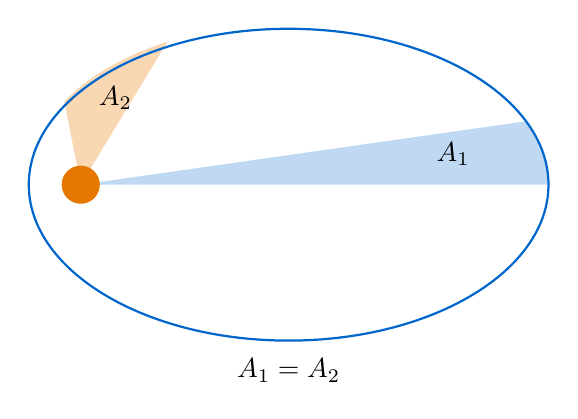
\begin{tikzpicture}[scale=1.1]
    \fill[spblue!25] (-2.4,0) -- (3,0) arc (0:24:3 and 1.8) -- cycle;
    \fill[sporange!30] (-2.4,0) -- (-1.4,1.65) arc (118:150:3 and 1.8) -- cycle;
    \draw[thick, spblue] (0,0) ellipse (3 and 1.8);
    \fill[sporange] (-2.4,0) circle (0.22);
    \node at (1.9,0.35) {$A_1$};
    \node at (-2.0,1.0) {$A_2$};
    \node[below] at (0,-1.9) {$A_1 = A_2$};
  \end{tikzpicture}
\end{frame}
\note{\L{%
  \begin{itemize}
    \item Near the Sun the planet moves faster
    \item Both areas take the same time
    \item Show it with the drawing tool
  \end{itemize}}{%
  \begin{itemize}
    \item In Sonnennähe bewegt sich der Planet schneller
    \item Beide Flächen brauchen die gleiche Zeit
    \item Mit dem Zeichenwerkzeug zeigen
  \end{itemize}}{%
  \begin{itemize}
    \item Près du Soleil, la planète va plus vite
    \item Les deux aires prennent le même temps
    \item Le montrer avec l'outil de dessin
  \end{itemize}}}

\begin{frame}{\L{Third law: period and distance}{Drittes Gesetz: Umlaufzeit und Abstand}{Troisième loi : période et distance}}
  \begin{columns}[c]
    \column{0.42\textwidth}
    \centering
    \Large $\displaystyle \frac{T^2}{a^3} = \text{const.}$
    \column{0.55\textwidth}
    \centering
    \begin{tabular}{lrrr}
      \toprule
      & $a$ (AU) & $T$ (\L{yr}{J.}{ans}) & $T^2/a^3$ \\
      \midrule
      \L{Mercury}{Merkur}{Mercure} & 0.387 & 0.241 & 1.00 \\
      Venus & 0.723 & 0.615 & 1.00 \\
      \L{Earth}{Erde}{Terre} & 1.000 & 1.000 & 1.00 \\
      Mars & 1.524 & 1.881 & 1.00 \\
      \L{Jupiter}{Jupiter}{Jupiter} & 5.203 & 11.86 & 1.00 \\
      \bottomrule
    \end{tabular}
  \end{columns}
\end{frame}
\note{\L{%
  \begin{itemize}
    \item The ratio is the same for every planet
    \item Newton later derived it from gravity
    \item Point at Jupiter: 12 years for one orbit
  \end{itemize}}{%
  \begin{itemize}
    \item Das Verhältnis ist für jeden Planeten gleich
    \item Newton leitete es später aus der Gravitation her
    \item Auf Jupiter zeigen: 12 Jahre für einen Umlauf
  \end{itemize}}{%
  \begin{itemize}
    \item Le rapport est le même pour chaque planète
    \item Newton l'a ensuite déduit de la gravitation
    \item Montrer Jupiter : 12 ans pour une orbite
  \end{itemize}}}

\begin{frame}{\L{The inner planets}{Die inneren Planeten}{Les planètes intérieures}}
  \centering
  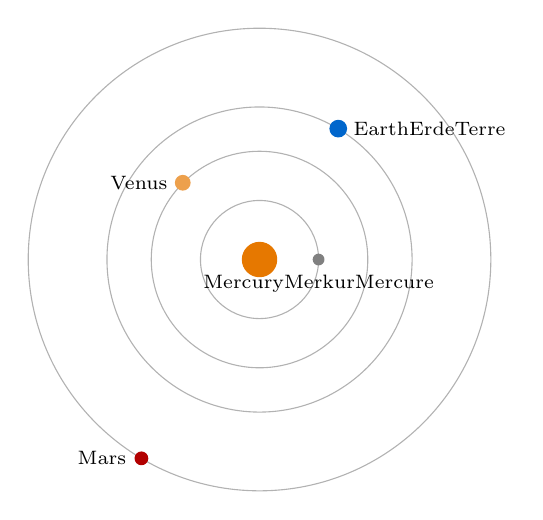
\begin{tikzpicture}[scale=1.25]
    \fill[sporange] (0,0) circle (0.18);
    \foreach \r in {0.6, 1.1, 1.55, 2.35} {
      \draw[gray!60] (0,0) circle (\r);
    }
    \fill[gray] (0.6,0) circle (0.06) node[below=2pt, font=\scriptsize, black] {\L{Mercury}{Merkur}{Mercure}};
    \fill[sporange!70] (-0.78,0.78) circle (0.08) node[left=2pt, font=\scriptsize, black] {Venus};
    \fill[spblue] (0.8,1.33) circle (0.09) node[right=2pt, font=\scriptsize, black] {\L{Earth}{Erde}{Terre}};
    \fill[red!70!black] (-1.2,-2.02) circle (0.07) node[left=2pt, font=\scriptsize, black] {Mars};
  \end{tikzpicture}
\end{frame}
\note{\L{%
  \begin{itemize}
    \item Orbits drawn to scale
    \item Mars has the most elliptical orbit of the four
  \end{itemize}}{%
  \begin{itemize}
    \item Bahnen maßstabsgetreu
    \item Mars hat die elliptischste Bahn der vier
  \end{itemize}}{%
  \begin{itemize}
    \item Orbites à l'échelle
    \item Mars a l'orbite la plus elliptique des quatre
  \end{itemize}}}

\begin{frame}{\L{Summary}{Zusammenfassung}{Résumé}}
  \begin{enumerate}
    \item \L{Orbits are ellipses with the Sun in one focus}{Bahnen sind Ellipsen mit der Sonne in einem Brennpunkt}{Les orbites sont des ellipses, le Soleil à un foyer}
    \item \L{Equal areas are swept in equal times}{In gleichen Zeiten werden gleiche Flächen überstrichen}{Des aires égales sont balayées en des temps égaux}
    \item $T^2 \propto a^3$ \L{for every planet}{für jeden Planeten}{pour chaque planète}
  \end{enumerate}
\end{frame}
\note{\L{Questions? Next week: Newton's law of gravitation.}{Fragen? Nächste Woche: Newtons Gravitationsgesetz.}{Des questions ? La semaine prochaine : la loi de la gravitation de Newton.}}

\end{document}
